A Figura~\ref{fig:faculdade} apresenta o modelo lógico do banco de 
dados {\tt FACULDADE}.

\begin{figure}[ht]
  \centering
  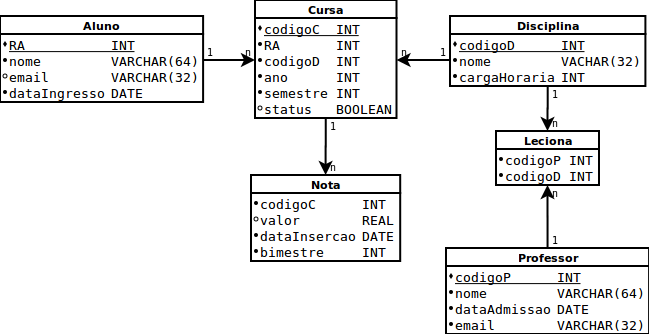
\includegraphics[scale=.6]{faculdade.png}
  \caption{Modelo lógico para o banco de dados {\tt FACULDADE}.}
  \label{fig:faculdade}
\end{figure}

As seguintes restrições devem ser aplicadas para os atributos:

\begin{itemize}

\item O campo {\tt RA} corresponde ao código do aluno, e é
  incrementado automaticamente a cada inserção de dados.
\item Na tabela {\tt Cursa}, o atributo {\tt semestre} é do tipo {\tt
    INT} e segue a seguinte convenção: {\tt 1} indica 1$^o$ semestre e
  {\tt 2} 2$^o$ semestre.
\item Na tabela {\tt Cursa}, o atributo {\tt status} é do tipo {\tt
    BOOLEAN} e segue a seguinte convenção: {\tt TRUE} significa
  aprovado, {\tt FALSE} reprovado e {\tt NULL} significa exame se a
  data atual for maior que a data de fechamento do semestre.  
\item Na tabela {\tt Nota}, o atributo {\tt bimestre} segue a seguinte
  convenção: o valor {\tt 1} significa 1$^o$~bimestre, {\tt 2}
  significa 2$^o$~bimestre e {\tt 3} significa exame.
\end{itemize}


\question{5}~Com base no modelo lógico da Figura~\ref{fig:faculdade},
crie as seguintes visões:

\begin{enumerate}[a)]
\item Liste o RA e nome todos os alunos que já estudaram com o
  professor ``Leosman Gusmão''; \ppoint{1}
\item  Liste o RA e nome de todos os alunos que já cursaram ``Cálculo''; \ppoint{1}
\item  Liste o nome de todos os professores que lecionaram a disciplina de
  ``Inglês''; \ppoint{1}
\item  Liste o RA todos os alunos que obtiveram nota menor que 5,0 no
  1$^o$ bimestre do 2$^o$ semestre de qualquer ano da disciplina de
  ``Estatística''. \ppoint{2}
\end{enumerate}
